\documentclass{article}
\usepackage{bm, amsmath,graphicx, subfigure, subfig, wrapfig, float, array, color}
\usepackage[plain]{algorithm}
\usepackage{algpseudocode, algorithmicx}
\usepackage{flexisym}
\usepackage{amsthm}
\usepackage{listings}
\usepackage{qtree}

\definecolor{MyDarkGreen}{rgb}{0.0,0.4,0.0}
\lstset{language=Matlab, 
basicstyle=\small\ttfamily,
commentstyle=\usefont{T1}{pcr}{m}{sl}\color{MyDarkGreen}\small}

\begin{document}

\title{sLBFGS+PLS Implementation Notes}
\author{Hammaad Adam, Chaitanya Rastogi and Tomas Rube}
\maketitle

\section{Notation, etc.}
\begin{itemize}
	\item $f$: the learning model we are trying to infer parameters for (objective function); $f(t) = \hat{\mathcal{L}}(x(t))$ 
	\item $t$: the current location; position vector is given by $x(t)$
	\item $y_t$, $y_t'$: noisy function and gradient values of $f$ at $t$
	\item $\sigma_f$, $\sigma_{f'}$: estimates of noise in function value and gradient
	\item $d$: the current line search direction
	\item $\odot$: element-wise operation, i.e. $x^{\odot 2}$ indicates element-wise squaring of the vector $x$, while $a\odot b$ indicates element-wise multiplication of the two vectors
\end{itemize}
The sLBFGS used in testing the code here was copied from my original Java code into Matlab. Testing has shown this version is not as efficient as the original Java code, probably due to some minor 0-1 array indexing issue in \texttt{twoLoopRecursion} that makes it slightly unstable. However, I still believe the overall trend of the results hold. 
\section{Scaling Issues}
A major component of the probabilistic line search (PLS) paper discussed the elimination of hyperparameters. Many of these parameters were used to set the intrinsic scale of the gaussian process (GP) surrogate function on which the line search optimization was taking place. Upon closer inspection, the implementation of some of these scaling parameters was not in line with the theoretical description in the paper and/or did not make sense in the context of sLBFGS. Correcting these scaling parameters was critical to the stability of the line search when used with sLBFGS and are discussed below.
\subsection{Scale factor $\beta$}
The scaling factor $\beta$ in the code and pseudocode is used to eliminate the hyperparameter $\theta$, which ``scales the prior variance'' according to the paper. By setting $\theta=1$ and rescaling the objective with $|y_0'|$, we get $y(0)=0$ and $y'(0)=-1$. In other words,
\begin{gather}
\label{eq:y_scaling} y_i = \frac{y_i - y_0}{|y_0'|} \\
\label{eq:dy_scaling} y_i' = \frac{y_i'}{|y_0'|}
\end{gather}
Clearly, $|y_0'|$ refers to the `norm of the gradient of $f$ at the start of the line search,' based off of the definitions used elsewhere in the paper. However, in the pseudocode for \texttt{probLineSearch} at line 15, the scaling factor $\beta$ is defined as
\[ \beta \leftarrow |d'\cdot \Sigma_{df_0}|,\]
where $d$ is the search direction and $\Sigma_{df_0}$ is the sample variances of the gradient. This is clearly wrong, and the code does not reflect this; rather, the Matlab code uses
\begin{center}
\texttt{beta = abs(search\_direction\textprime*df0);}
\end{center}
where \texttt{df0} is the function gradient at the origin of the line search. While this statement is congruent with the definition in the text of the paper for SGD, it is \emph{not} for BFGS methods. The reason lies in the definition of the search direction $d$ for both methods:
\[ \text{SGD: } d=-\nabla f \]
\[\text{BFGS: } d=-H^{-1}\nabla f \]
where $H$ is the pseduo-hessian matrix computed in the BFGS updates. As such, beta in the two cases becomes
\[ \text{SGD: } \beta=|(-\nabla f)' \cdot \nabla f | = |y_0'|\]
\[\text{BFGS: } \beta=|(-H^{-1}\nabla f)' \cdot \nabla f| \neq |y_0'| \]
In the case of BFGS updates, it is possible that the above definition of $\beta$ can be $\approx 0$, as the inverse hessian can rotate the gradient vector to be nearly orthogonal to the gradient. The correct code should be 
\begin{center}
\texttt{beta = norm(df0);}
\end{center}
Fixing this rescaling greatly enhances the stability of the GP: before this fix, running sLBFGS + PLS with a batchsize of 20 and epoch period of 50 steps resulted in $\beta$ values approaching $10^{-9}$.
\subsection{Rescaling by $\alpha_0$}
$\alpha_0$ is the initial step size in the line search, in non-dimensional units. In the theoretical discussion of the scaling factor $\beta$, we see that \eqref{eq:y_scaling} and \eqref{eq:dy_scaling} only admit the norm of the function gradient. Similarly, we see that the paper discusses rescaling the noise estimates for $\sigma_f$ and $\sigma_{f'}$ as follows:
\begin{gather}
\label{eq:sy_scaling} \sigma_f = \frac{\sigma_f}{|y'(0)|} \\
\label{eq:sdy_scaling} \sigma_{f'} = \frac{\sigma_{f'}}{|y'(0)|}
\end{gather}
Curiously, the pseudocode for \texttt{probLineSearch} at lines 15 and 16 instead show:
\[ \sigma_f \leftarrow \sqrt{\Sigma_{f_0}}/(\alpha_0\cdot\beta) \]
\[ \sigma_{df} \leftarrow \sqrt{(d^{\odot 2})'\cdot \sigma_{df_0})} \]
In addition, the pseudocode for \texttt{evaluateObjective} at lines 6 and 7 show:
\[ y \leftarrow (y-f_0)/(\alpha_0\cdot\beta) \]
\[ dy \leftarrow (dy' \cdot d)/\beta \]
The original Matlab code follows this convention as well. It is unclear why the initial step size is needed to rescale the function values and gradients, especially as it is not motivated in the text. In fact, given that function values $y$ and noise $\sigma_f$ are scaled by an additional $1/\alpha_0$ term, we can get improperly scaled function value estimates relative to gradient estimates. In the sLBFGS setting, where a fixed $\alpha_0=.1$ was used, this translates to an order of magnitude variation. As such, the Matlab code was amended as follows:
\begin{center}
\texttt{sigmaf  = sqrt(var_f0)/beta; (in probLineSearch)}\\
\texttt{y = (y - f0)/beta; (in evaluate_function)} \\
\texttt{y_tt = y*beta + f0; (in make_outs)}
\end{center}
\subsection{Step Size Selection}
In traditional BFGS methods, the quasi-newton nature of these methods generate `properly' scaled search directions that allow the initial step size of the line search, $\alpha_0$, to be set to 1 every iteration. Significantly, this value is independent of the objective function being optimized. In contrast, the original sLBFGS implementation uses a fixed step size $\eta$ that needs to be optimized to suit the objective at hand. In yet another variation, the original PLS approach removes the need to tune the initial step size by setting it to 1, but relies on ad-hoc schemes that track the size of previous steps to change the step size of the upcoming iteration. Thankfully, these updating schemes are unnecessary in the sLBFGS + PLS setting, where $\alpha_0 = \eta$. While an improvement, it is surprising how the sLBFGS + PLS method cannot deal with objective-independent unitary step sizes without running into convergence issues. 
\section{Noise Estimation}
Another major theoretical component of the PLS paper is the usage of noisy estimates to do a somewhat deterministic optimization of an objective function. As such, determining the noise level of these estimates forms a critical component of the PLS. However, I believe there is a major approximation made in the paper that can significantly impact the performance of the line search, especially within the context of stochastic variance-reduced gradients (SVRG). 

The original PLS implementation sets the function and gradient noise levels ($\sigma_f$ and $\sigma_{f'}$) at the \emph{start} of the line search, i.e. at $t=0$, and maintains it throughout the search. Surprisingly, faster convergence was observed in the SGD setting when the code was modified to change $\sigma_f$ and $\sigma_{f'}$ to the largest value encountered during the line search. This test highlighted the impact of the approximation in estimating the variance. 
\subsection{SEM in the Minibatch Setting}
The problem in estimating the SEM of function and gradient values in a mini-batch can be recast into a toy problem:
\begin{quote}
Let us begin with a set of points $A$, which have mean $\mu_A$, variance $\sigma_A^2$, and SEM $\sigma_A/\sqrt{|A|}$, where $|A|$ is the cardinality of the set $A$. Our goal is to estimate $\mu_A$; however, we only have access to sets $A'$ that are generated by sampling points (without replacement) from $A$ such that $|A'| \leq |A|$. If we can only observe sets $A'$, what is the SEM of the means $\mu_{A'}$ that we observe?
\end{quote}
Conceptually, this toy problem is key to understanding the error in the process for estimating the function and gradient SEMs in the current approach. When a mini-batch is used to \emph{estimate} function and gradient values, we know the means have some spread (SEM) around the true function and gradient means as computed \emph{exactly} on the entire dataset. As such, in the limit where my mini-batch hits the full size of the dataset, there should be \emph{no} variance in the function and gradient means. The current approach employed in the paper and the code uses a naïve algorithm to compute the variance, using Bessel's correction:
\begin{gather}
\label{eq:sf} \sigma_f^2 = \frac{1}{n}\frac{n}{n-1} \left[\frac{1}{n} \sum_{i\in A'} \ell^2(A_i) - \left(\frac{1}{n} \sum_{i\in A'} \ell(A_i) \right)^2 \right] \\
\label{eq:sdf} \sigma_{f'}^2 = \frac{1}{n}\frac{n}{n-1} d^{\odot 2} \cdot \left[ \frac{1}{n} \sum_{i \in A'} \nabla \ell(A_i)^{\odot 2} - \left(\frac{1}{n} \sum_{i \in A'} \nabla \ell(A_i) \right)^{\odot 2} \right]
\end{gather}
where $N=|A|$ and $n=|A'|$. Unfortunately, this naïve method computes non-zero estimates of $\sigma_f$ and $\sigma_{f'}$ when $A' = A$. If we have access to the `true' $\sigma_A$ of the whole set (i.e. the intrinsic variance), Tomas proposed the following correction to estimate mini-batch SEM:
\begin{equation}
\label{eq:Tomas_correction}
\text{SEM}_{A'} = \sqrt{\frac{N-n}{Nn} \sigma_A^2},
\end{equation}
The derivation is presented below. 
\begin{proof}
Consider $N$ random variables $x_i$, where $i\in 1,\ldots,N$ drawn from a distribution with variance $\sigma^2$. The average of these variables is then 
\[ \mu_N = \frac{1}{N}\sum_i^N x_i \]
If you can only use the first $n$ variables to estimate the mean, we get 
\[ \mu_n = \frac{1}{n}\sum_i^n x_i \]
Let 
\[\mu_{N-n} = \frac{1}{N-n}\sum_{i=n+1}^N x_i\]
Then
\[ \mu_N = \frac{n \mu_n + (N-n)\mu_{N-n}}{N} \]
We can define the error $e$ in estimating $\mu_N$ using $\mu_n$ as
\[ e(n|N) = \mu_N-\mu_n = \frac{n\mu_n + (N-n)\mu_{N-n}}{N}-\mu_n = \frac{N-n}{N}(\mu_{N-n}-\mu_n)\]
The variance of this error is then 
\begin{align*}
\text{Var}[e(n|N)] &= \frac{(N-n)^2}{N^2}\left( \text{Var}[\mu_{N-n}] - \text{Var}[\mu_n] \right) \\
&= \frac{(N-n)^2}{N^2} \left(\frac{1}{N-n} +\frac{1}{n} \right) \sigma^2 \\
&= \frac{N-n}{Nn}\sigma^2
\end{align*}
\end{proof}
\subsection{Other Variance Measures}
Tomas suggested an alternative method for measuring the SEM of the gradient: 
\begin{equation}
\label{eq:sdf_tomas} \sigma_{f'}^2 = \frac{1}{n}\frac{n}{n-1} \left[ \frac{1}{n} \sum_{i \in A'} \left[d \cdot \nabla \ell(A_i) \right]^{\odot 2} - \left(\frac{1}{n} \sum_{i \in A'} d\cdot\nabla \ell(A_i) \right)^{\odot 2} \right]
\end{equation}
Conceptually, this modification captures the per-data point gradient variance in the \emph{direction} of descent rather than the projection of the gradient SEM on the descent direction. When tested in place of the original estimator in a SGD context, the PLS was more efficient.
\section{PLS in the SVRG Setting}
Stochastic Variance Reduced Gradient, or SVRG, is a method used to improve the speed and efficiency of convergence in stochastic optimization methods. Originally designed for use in the SGD context, it was ported to the quasi-newton setting in sLBFGS. SVRG is supposed to reduce the `variance' of the SGD estimates through a modified update scheme that relies on a gradient $\mu_k$ that is computed on the entire dataset once per epoch at some position $x_k$. The SVRG gradient at every iteration $i$ on mini-batch $b$ is then
\begin{equation}
\label{eq:svrg}
\nabla_{\text{SVRG}} f(x_i, b) = \underbrace{\nabla f(x_i, b)}_{\substack{\text{stochastic} \\ \text{estimate}}} - \underbrace{(\nabla f(x_k, b) - \mu_k)}_{\text{batch bias}}
\end{equation}
where $\nabla f(x_k, b)$ indicates the gradient of $f$ at $x_k$ as computed on mini-batch $b$. In my understanding, this update estimates the batch-induced bias in stochastic estimates by comparing the difference between the gradient computed on the full dataset and the mini-batch $b$ at $x_k$. This difference represents the bias induced by computing on batch $b$ and can be subtracted from the current estimate of the gradient. As a result, the mean function and gradient values as estimated from the mini-batch should be closer to the true values.
\subsection{Scaling to SVRG Space}
Every sLBFGS update already computes the SVRG gradient estimate $v_t$ every iteration. In order to properly run the line search in SVRG space, the starting function values need to be adjusted as well:
\begin{lstlisting}
for k = 0:maxEpoch
	...
	% function and gradient on the full dataset
	[fFull, mu_k] = f(w_k);
	...
	% iterations within an epoch
	for t = 1:m
		% select batchsize 
		sidx = randsample(1:N, batchsize);
		% compute on minibatch
		[f_xt, grad_xt] = f(x_t, sidx);
		[f_wk, grad_wk] = f(w_k, sidx);
		% compute SVRG function and grad
		f_t = (f_xt + fFull) - f_wk;
		v_t = (grad_xt + mu_k) - grad_wk;
		...
		% compute effective direction
		if (r < 1)
			% no hessian updates have occured
			effGrad = v_t;
		else
			effGrad = twoLoopRecursion(v_t);
		end
		...
		% use line search
		if (r < 1)
			step_size = ls(x_t, f_t, v_t, ...
			-effGrad, eta/norm(v_t), ..., 
			fFull, mu_k, w_k);
		else
			step_size = ls(x_t, f_t, v_t, ...
			-effGrad, eta, fFull, mu_k, ...
			w_k);
		end
\end{lstlisting}
In addition, \texttt{evaluate_function} in the probabilistic line search needs to be modified:
\begin{lstlisting}
% select batchsize
sidx = randsample(1:N, batchsize);
% compute on minibatch
[y_t, dy] = f(x0 + tt*alpha0*search_direction, sidx);
[y_k, grad_wk] = f(w_k, sidx);
y = (y_t + fFull) - y_k;
dy = (dy + mu_k) - grad_wk;
\end{lstlisting}
It is critical that the \emph{same} mini-batch is used to compute function and gradient values at $x_t$ and $w_k$. Doing so on different batches ruins the impact of bias reduction. When improperly implemented, the improper SVRG updates cause high-frequency, low-amplitude oscillations around the minimum, preventing convergence.
\subsection{Variance in the SVRG Context}
Just as both the function and gradient values input into the PLS need to be updated to remain in SVRG space, we need to ensure that SVRG variance is properly estimated. To understand how to approach this problem, let us look at the SVRG function update:
\[ f(x_t)_{\text{SVRG}} = f(x_t, b) - f(x_k, b) + f(x_k, N) \]
where $f(x_k, N)$ is the function value at $x_k$ computed on the full dataset. Then, the variance of this estimate is
\begin{equation}
\label{eq:svrg_var}
\text{Var}[f(x_t)_{\text{SVRG}}] = \text{Var}[f(x_t,b)] + \text{Var}[f(x_k, b)] - 2\,\text{Cov}(f(x_t),f(x_k))
\end{equation}
as the function value computed on the full batch has no variance. Estimating the covariance term is difficult analytically, so we can (conservatively) estimate it with the following methods:
\begin{itemize}
	\item \textbf{Scale by $\sqrt{2}$:} $\text{Cov}=0$ and $\text{Var}[f(x_k, b)]=\text{Var}[f(x_t, b)]$
	\item \textbf{Rescaled Full-Batch Estimate:} \\ $\text{Cov}=0$ and $\text{Var}[f(x_k, b)]=$ $\text{Var}[f(x_t, b)] =$ $(N-n)/N\cdot\text{Var}[f(x_k, N)]$
	\item \textbf{Full Computational Evaluation:} Evaluate $\text{Var}[f(x_t, b) - f(x_k,b)]$ every iteration
\end{itemize}
Depending on the methodology chosen, we can substitute the naïve gradient variance estimator \eqref{eq:sdf} with Tomas's more accurate one \eqref{eq:sdf_tomas}. The estimators shown above were tested in actual sLBFGS runs on the SVM test case for different batch sizes (Figs. \ref{fig:var_20} and \ref{fig:var_200}). In these plots, the `Scale by $\sqrt{2}$' option is not shown as it is a trivial case that would result in a shifted $x_t$ track. Here, we can see that the rescaled full-batch estimate quite accurately captures the variance in the $x_t$ and $w_k$ estimates, especially in the iterations closer to convergence. It should be noted that the displayed $x_t$ and $w_k$ tracks show 11-iteration moving averages - this is to average out fluctuations roughly 3-5 orders of magnitude between successive estimates.
\begin{figure}[h]
\centering
\subfigure[SVM Function Variance]{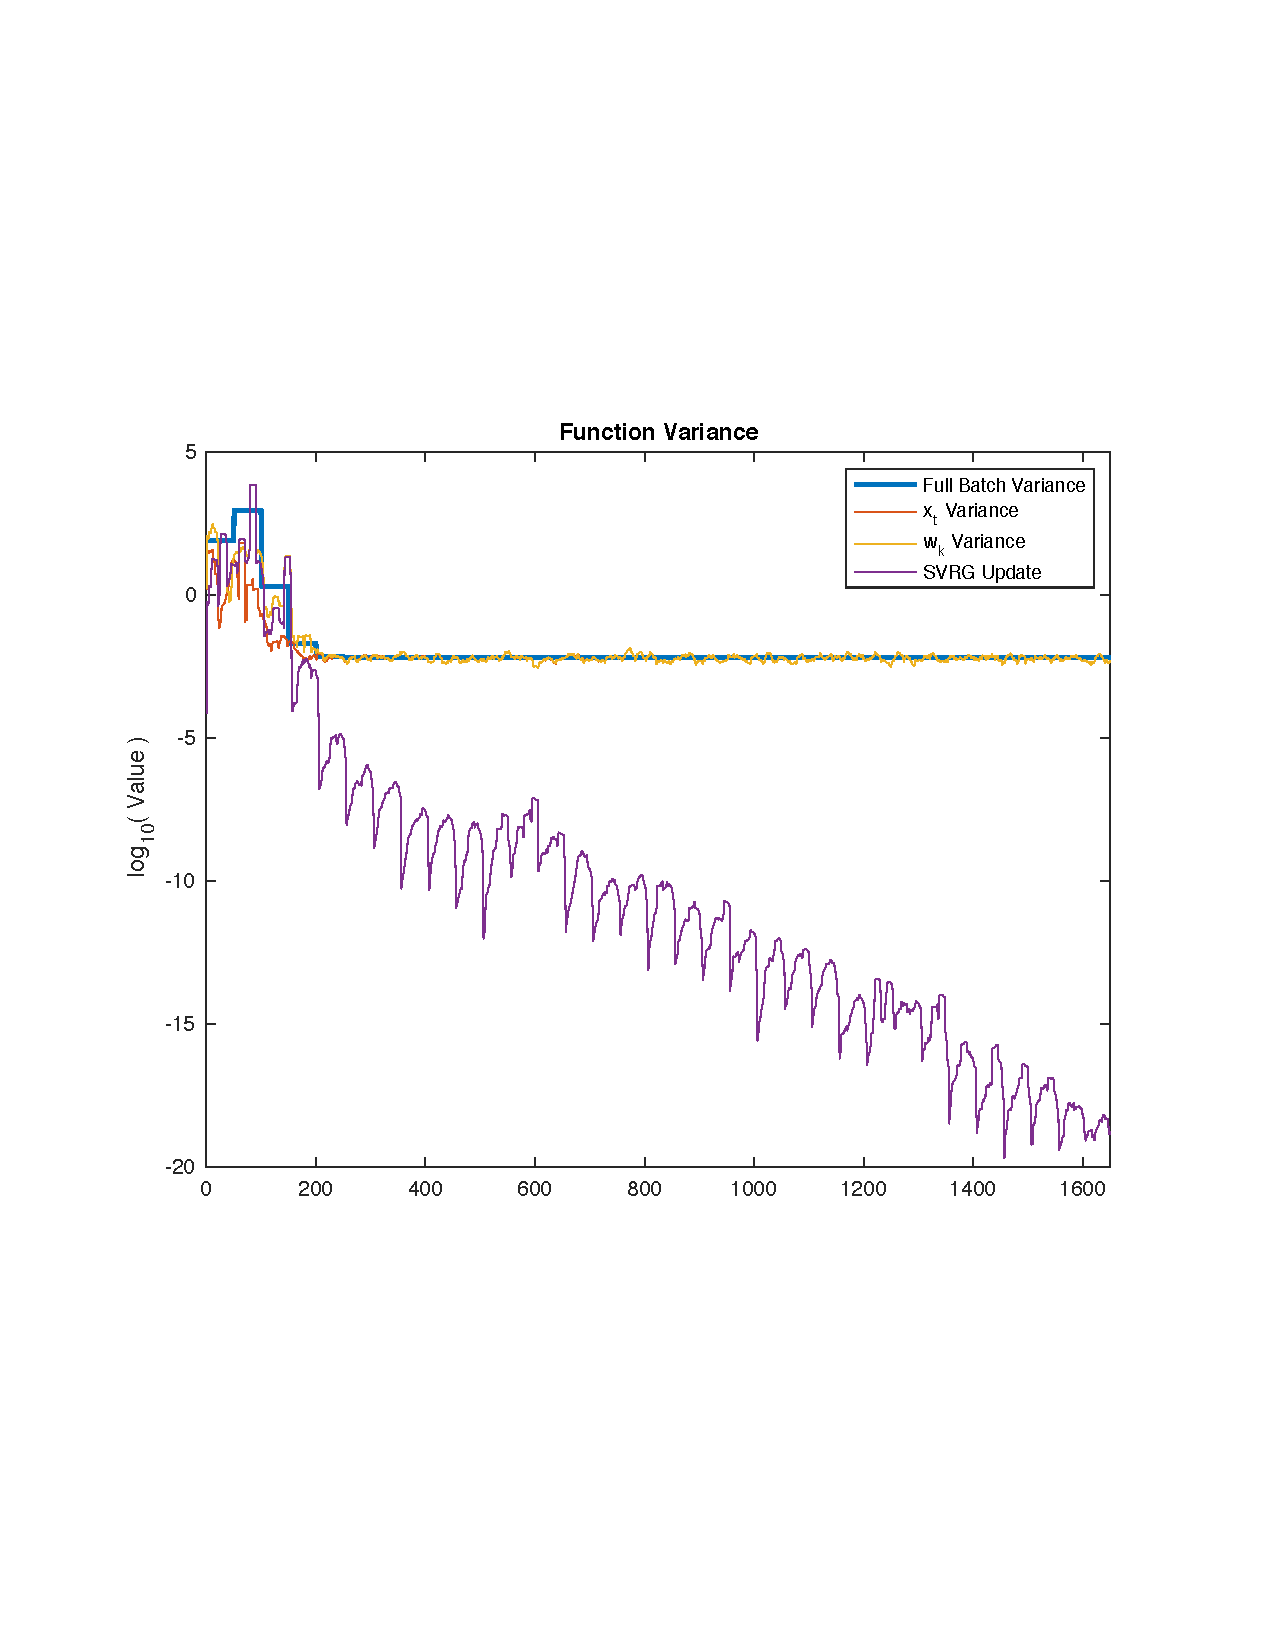
\includegraphics[width=.45\linewidth]{svm_func_var_20.pdf}}
\subfigure[SVM Gradient Variance]{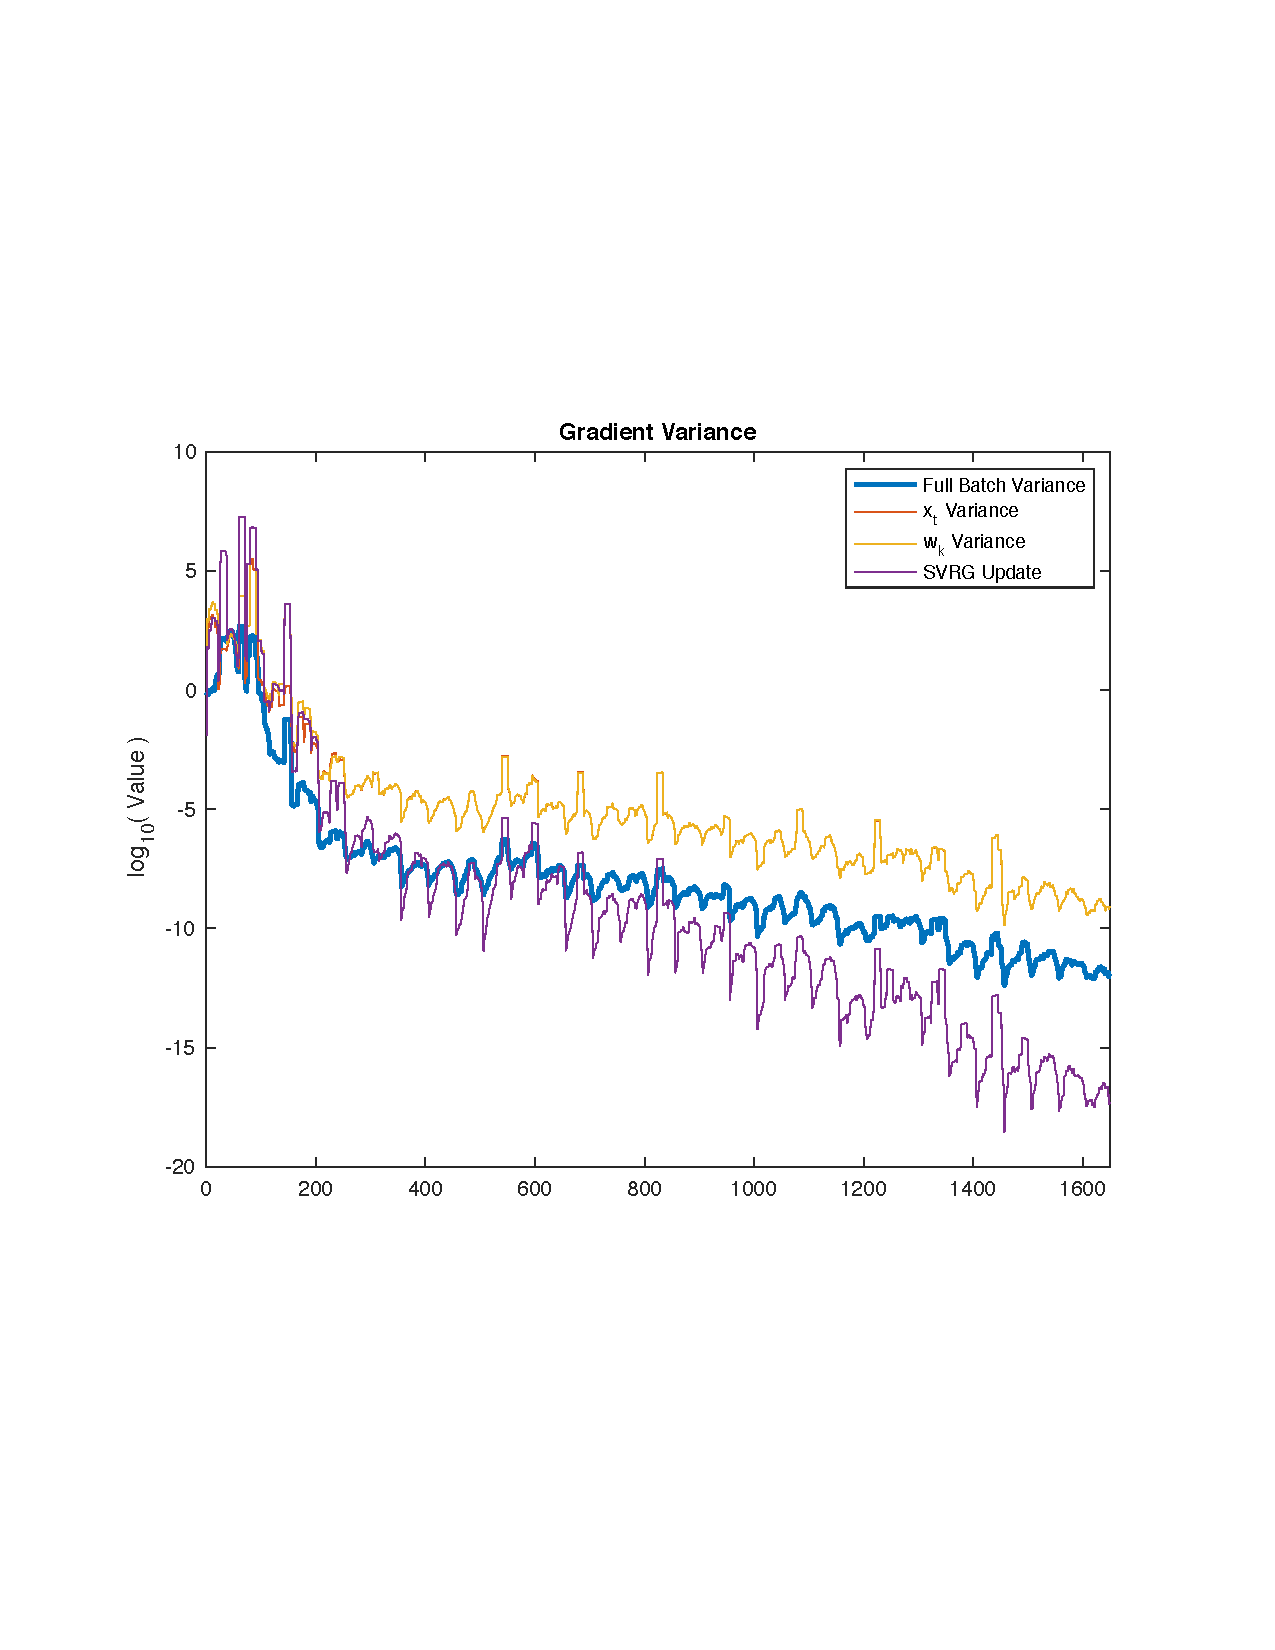
\includegraphics[width=.45\linewidth]{svm_grad_var_20.pdf}}
\caption{Function and Gradient Variances for the SVM test case with a gradient batch size of 20, a hessian batch size of 200, a hessian update period of 10 iterations, and a full gradient computation (an epoch) every 50 iterations. 11 step moving averages are shown for all tracks except for the full batch function variance track. X-axis shows the number of iterations. The full batch variance values use Tomas's SEM correction term.}
\label{fig:var_20}
\end{figure}
\begin{figure}[h!]
\centering
\subfigure[SVM Function Variance]{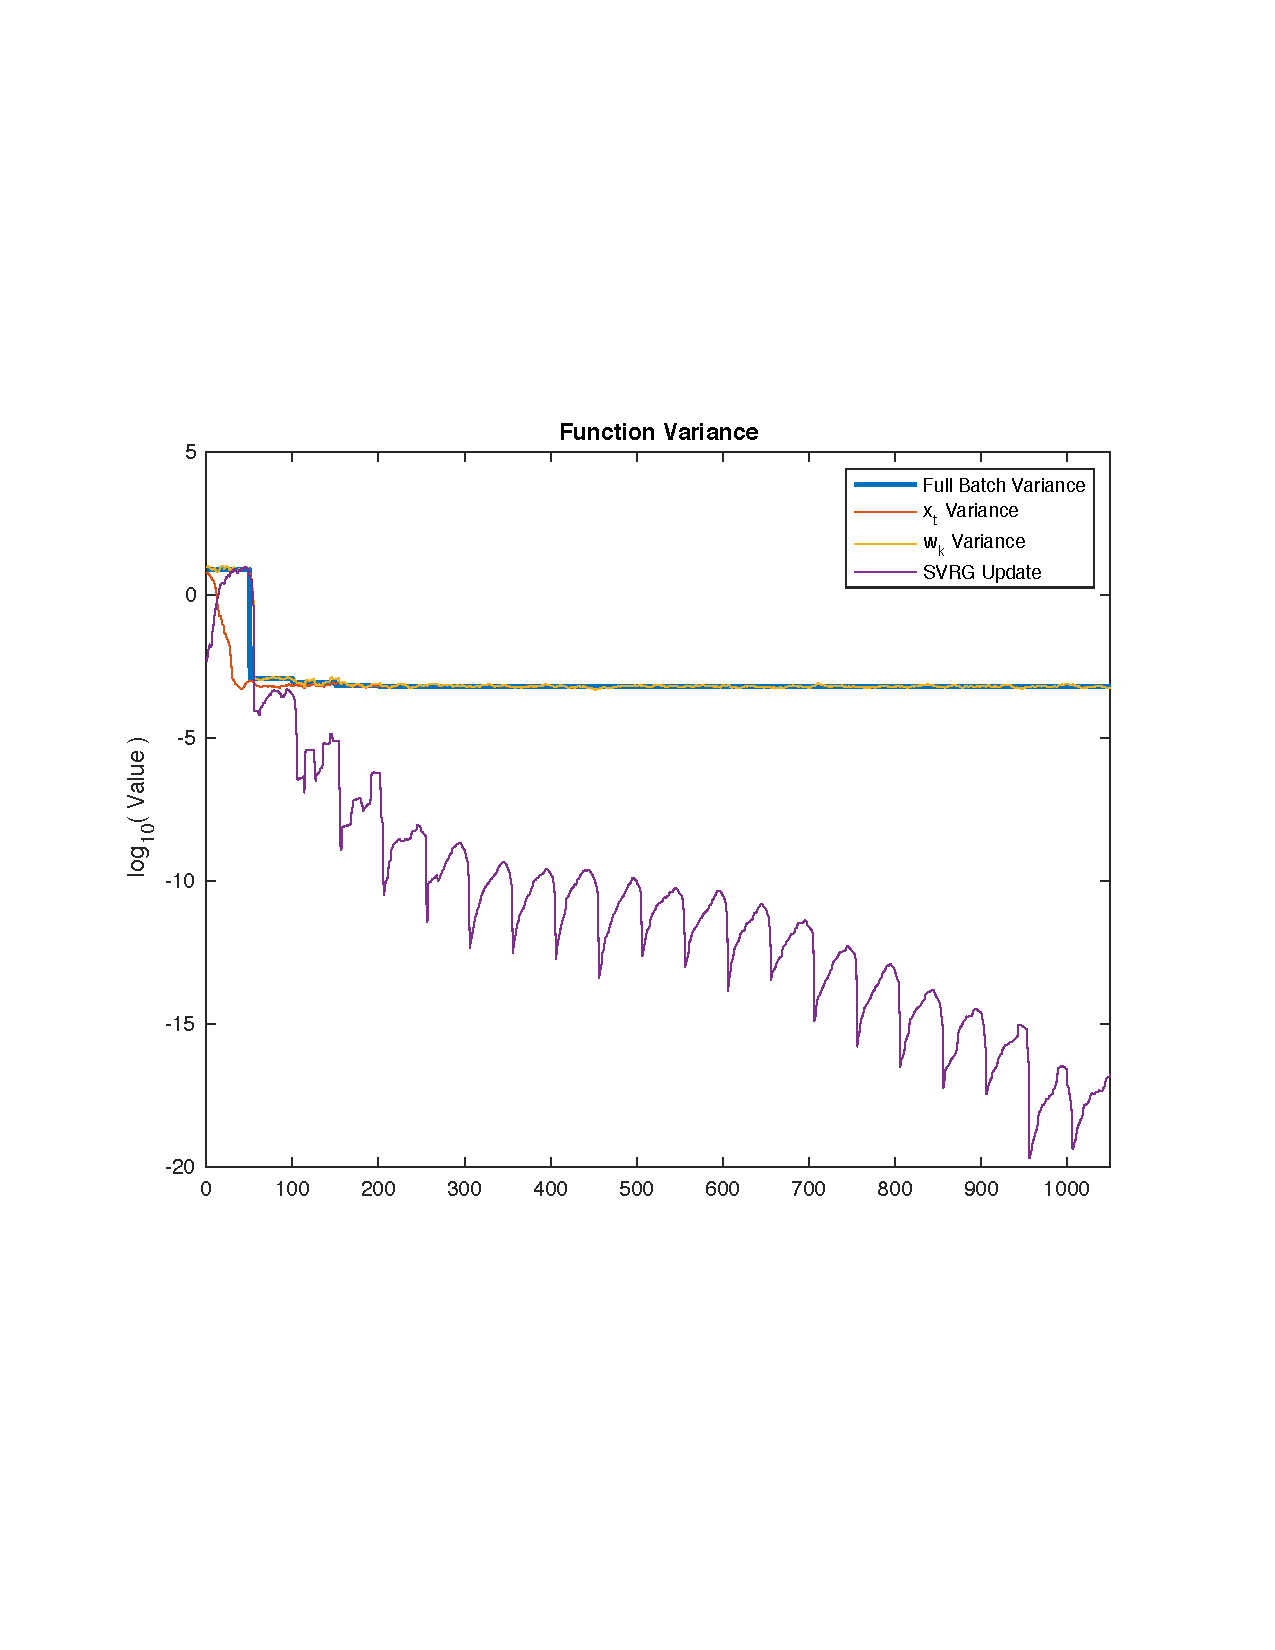
\includegraphics[width=.45\linewidth]{svm_func_var_200.pdf}}
\subfigure[SVM Gradient Variance]{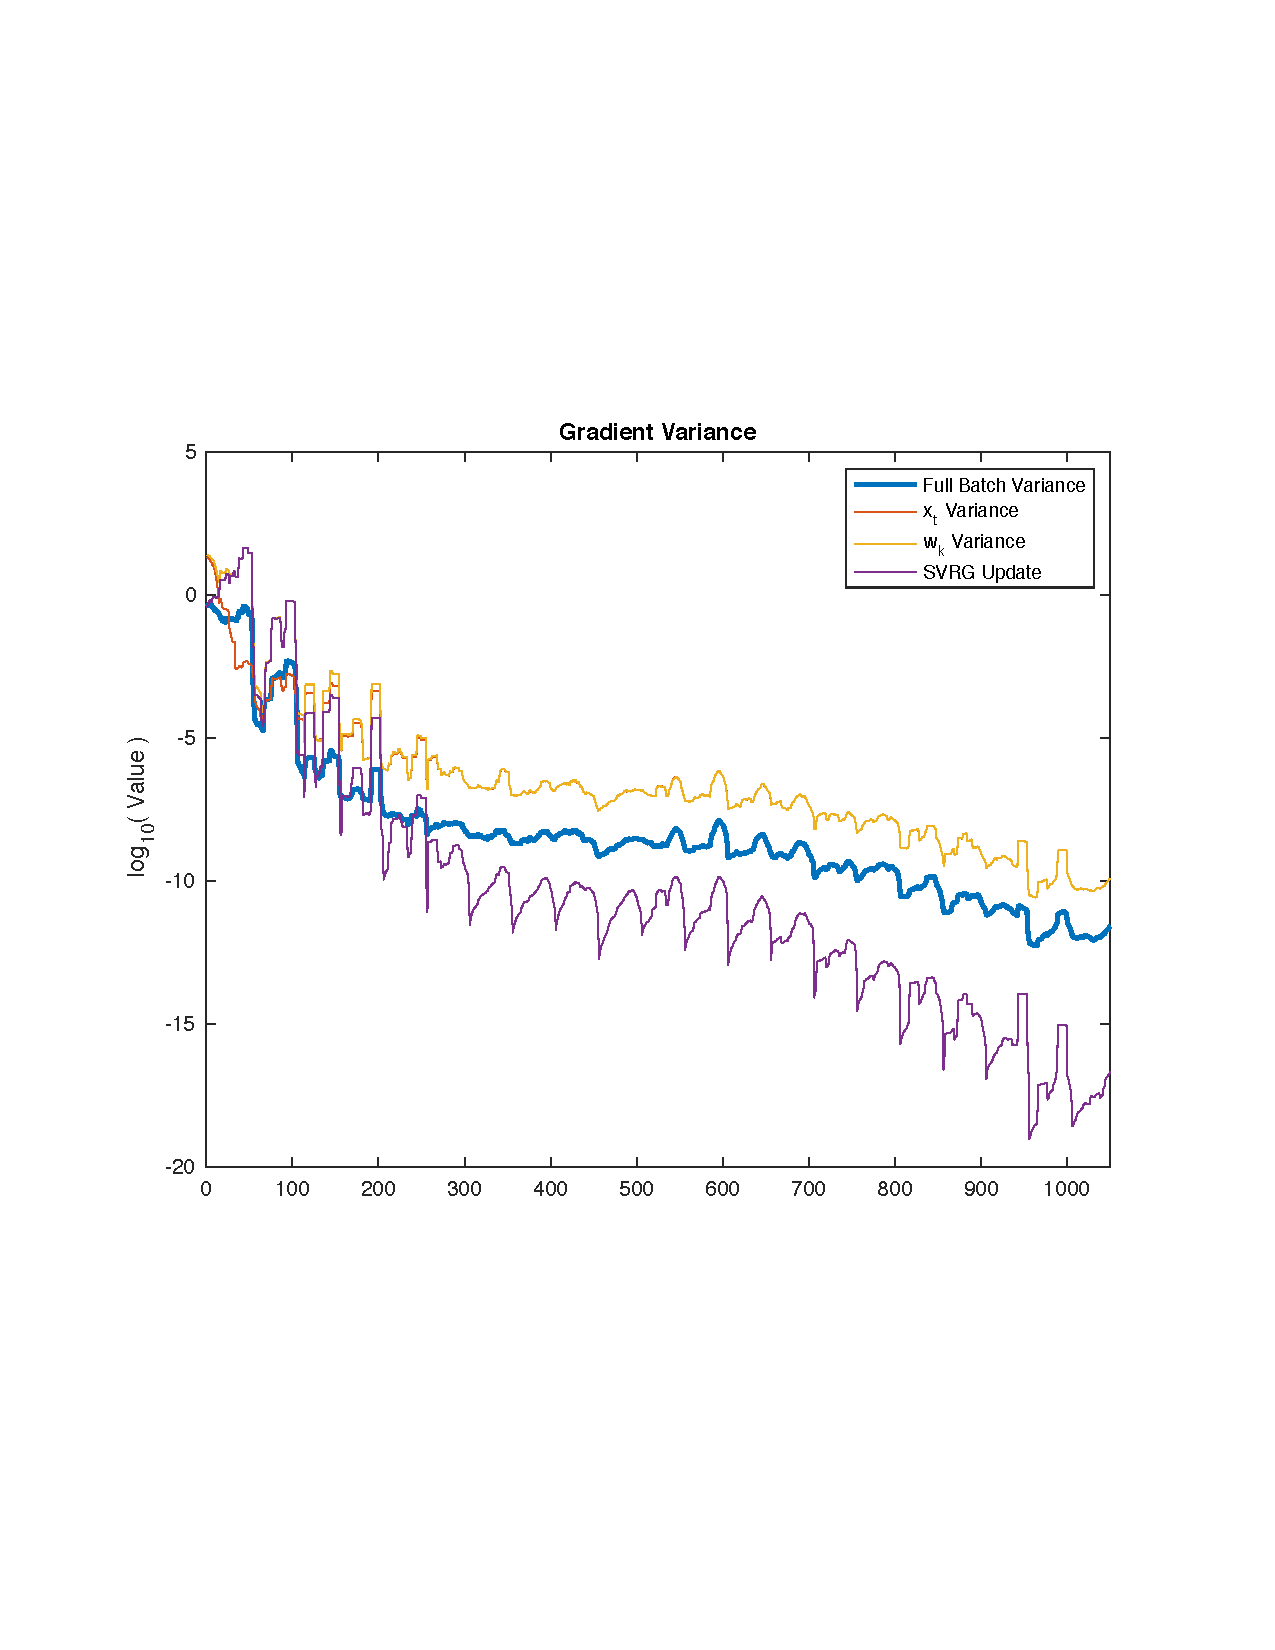
\includegraphics[width=.45\linewidth]{svm_grad_var_200.pdf}}
\caption{Function and Gradient Variances for the SVM test case with a gradient batch size of 200, a hessian batch size of 2000, a hessian update period of 10 iterations, and a full gradient computation (an epoch) every 50 iterations. 11 step moving averages are shown for all tracks except for the full batch function variance track. X-axis shows the number of iterations, and the full batch variance values use Tomas's SEM correction term.}
\label{fig:var_200}
\end{figure}
Surprisingly, we see that the direct calculation of the SVRG update results in incredibly low variances, especially towards convergence. This is largely due to the fact that the distance between successive sLBFGS iterations drops as the optimizer closes in on a minimum. As such, we should expect the distance between $x_t$ and $w_k$ to decrease over time and result in similar function and gradient estimates at $x_t$ and $w_k$. Therefore, it seems safe to ignore the SVRG track as an artifact. 

In summary, it appears that the rescaled full-batch estimate should be the most robust noise estimator. However, this would make evaluating Tomas's improved estimator computationally intensive. It appears that the reduced bias and improved efficiency would not outweigh the computational costs. Given that a function call can compute the naïve SEM estimators, we can implement this improvement easily:
\begin{lstlisting}
% SVRG step
[fFull, mu_k, fVar_f, fVar_df] = func(w_k);
....
% Evaluate line search
ls_function(..., fVar_f*(N-n)/N, fVar_df*(N-n)/N,...)
\end{lstlisting}

\section{Determining the `Suitability' of the Descent Direction}
\subsection{Metrics for GP Precision and Recall}
Discuss tree structure.

\begin{center}
\Tree[.$d\cdot\nabla f<0$? 
		[.{Yes. Did PLS correctly\\ identify the direction?} 
			[.{Yes.\\$f_{i+1}<f_i$?} 
				[.Yes. \rotatebox{85}{\parbox{3.5cm}{\raggedleft CDCLFD: \\ BFGS+LS Success}} ]
				[.No. \rotatebox{85}{\parbox{3.5cm}{\raggedleft CDCLFI:\\accidentally overshot}} ]]
               		[.{No.\\$f_{i+1}<f_i$?} 
				[.Yes. \rotatebox{85}{\parbox{3cm}{\raggedleft CDILFD: \\partial LS failure}} ] 
				[.No. \rotatebox{85}{\parbox{3cm}{\raggedleft CDILFI: \\ LS failure}} ]]]
		[.{No. Did PLS correctly \\ identify the direction?} 
			[.{Yes.\\$f_{i+1}<f_i$?} 
				[.Yes. \rotatebox{85}{\parbox{3cm}{\raggedleft IDCLFD:\\LS rescue}} ]
				[.No. \rotatebox{85}{\parbox{3cm}{\raggedleft IDCLFI: \\partial LS rescue}} ]]
               		[.{No.\\$f_{i+1}<f_i$?} 
				[.Yes. \rotatebox{85}{\parbox{3.5cm}{\raggedleft IDILFD: \\dumb luck: went \\ backward over a hill}} ] 
				[.No. \rotatebox{85}{\parbox{3cm}{\raggedleft IDILFI: \\total failure}} ]]]]
\end{center}
\subsection{`Small Step Size' Selection}
Discuss how small step size should be increased compared to the base PLS one. sLBFGS gets the direction right most of the time
\section{Alternative Line Search Candidate Methods}
ugh
\section{Condition Number and Null Space}
We know that both NRLB and ProBound have a large null space - this is the result of using an overparameterized representation for PWMs (for example, we infer $\Delta\Delta$G parameters for \{A, C, G, T\} at every position, while the `true' space has only 3 parameters). After Hammaad's group meeting presentation, Harmen suggested that we look into the effect of a large null space has on gradient-based optimization algorithms. 
\subsection{Impact of the Null Space}
For a general likelihood function $\mathcal{L}$, we can identify and remove the null space by computing either the eigendecomposition or SVD of the hessian at any (reasonable) point in the functional space. From experience, SVD was used as it was more stable for matrices with a high condition number (which we have). In addition, we can estimate the hessian with gradients using finite difference methods. Assuming we have this, the following Matlab code can be used to construct a projection matrix $\mathbf{U}$ that allows the projection of position and gradient vectors to and from the full space to the reduced space. 
\begin{lstlisting}
[UMat, SMat, ~] = svd(fdHessian);
U = UMat(:,(diag(SMat)>ev_cutoff));
\end{lstlisting}
Equivalent code can be constructed in Java with the JAMA package. Some things to note:
\begin{itemize}
\item In some cases (such as the SVM test case used here), the true null vectors can be found via SVD on the data matrix as well, and should, in general, be more stable. In practice, this makes no difference, as long as $\texttt{ev_cutoff}$ and the finite difference step size are appropriately chosen. 
\item It is \textbf{extremely} important to remove any regularization in $\mathcal{L}$ while identifying the null vectors. Regularization transforms rank-deficient problems into full-rank ones (see discussion below) and can prevent the identification of the null vectors. For simple regularization such as the $L^2$ norm, the following can be used to identify the null vectors:
\begin{lstlisting}
U = UMat(:,(diag(SMat)-lambda>ev_cutoff));
\end{lstlisting}
where \texttt{lambda} is the strength of the regularization. 
\end{itemize}
$\mathbf{U}$ can be used to convert between the full and reduced space as follows: 
\begin{table}[h!]
\centering
\begin{tabular}{c|c}
\begin{tabular}[c]{@{}c@{}}Full\\ Space\end{tabular} & \begin{tabular}[c]{@{}c@{}}Reduced\\ Space\end{tabular} \\[7pt] \hline 
$x^{F}$                                              & $\mathbf{U'}\,x^F$                                        \\
$\mathbf{U}\,x^{R}$                                  & $x^{R}$                                                
\end{tabular}
\end{table}

\noindent As the Java sLBFGS implementation is known to perform better than the Matlab version, it was augmented to allow optimization in the reduced space. This implementation was robustly tested with various parameter settings (Table \ref{table:nullspace}) and demonstrated that projecting out the null space had no impact on the optimizers. Interestingly, removing the regularization made it much harder for sLBFGS to converge.
\begin{table}[h]
\centering
\begin{tabular}{c|c|c|c|c|c|c|c}
\rotatebox{90}{\parbox{1.5cm}{Reduced \\ Space}} & $\lambda$ & \rotatebox{90}{\parbox{1.5cm}{Gradient \\ Batch}} & \rotatebox{90}{\parbox{1.5cm}{Hessian \\Period}} & \rotatebox{90}{\parbox{1.5cm}{Stoch.\\ Iters}} & \begin{tabular}[c]{@{}c@{}}Data Loops\end{tabular} & Epochs          & \rotatebox{90}{Failed} \\ \hline
F & $ 0.001 $ & $ 20 $ & $ 10 $ & $ 50 $ & $ 36.75 \pm 1.41 $ & $ 31.84 \pm 1.26 $ & \\
T & $ 0.001 $ & $ 20 $ & $ 10 $ & $ 50 $ & $ 36.85 \pm 1.51 $ & $ 31.93 \pm 1.34 $ & \\
F & $ 0 $ & $ 20 $ & $ 10 $ & $ 50 $ & N/A & N/A & 100 \\
T & $ 0 $ & $ 20 $ & $ 10 $ & $ 50 $ & $ 212.10 $ & $ 188 $ & 99 \\
F & $ 0.001 $ & $ 20 $ & $ 5 $ & $ 10 $ & $ 76.64 \pm 5.50 $ & $ 72.95 \pm 5.30 $ & \\
T & $ 0.001 $ & $ 20 $ & $ 5 $ & $ 10 $ & $ 75.64 \pm 3.49 $ & $ 71.99 \pm 3.36 $ & \\
F & $ 0 $ & $ 20 $ & $ 5 $ & $ 10 $ & $ 784.03 \pm 163.39 $ & $ 755.2 \pm 157.58 $ & 95 \\
T & $ 0 $ & $ 20 $ & $ 5 $ & $ 10 $ & $ 785 $ & $ 756 $ & 99 \\
F & $ 0.001 $ & $ 200 $ & $ 10 $ & $ 50 $ & $ 45.21 \pm 2.04 $ & $ 19.84 \pm 0.91 $ & \\
T & $ 0.001 $ & $ 200 $ & $ 10 $ & $ 50 $ & $ 45.08 \pm 1.53 $ & $ 19.78 \pm 0.69 $ & \\
F & $ 0 $ & $ 200 $ & $ 10 $ & $ 50 $ & $ 466.01 \pm 235.69 $ & $ 208.67 \pm 105.76 $ & 97 \\
T & $ 0 $ & $ 200 $ & $ 10 $ & $ 50 $ & $ 401.02 \pm 7.88 $ & $ 179.5 \pm 3.54 $ & 98 \\
F & $ 0.001 $ & $ 200 $ & $ 5 $ & $ 10 $ & $ 93.57 \pm 6.23 $ & $ 67.64 \pm 4.55 $ & \\
T & $ 0.001 $ & $ 200 $ & $ 5 $ & $ 10 $ & $ 93.51 \pm 6.51 $ & $ 67.6 \pm 4.76 $ & \\
F & $ 0 $ & $ 200 $ & $ 5 $ & $ 10 $ & $ 413.18 \pm 163.99 $ & $ 301.18 \pm 119.83 $ & 1 \\
T & $ 0 $ & $ 200 $ & $ 5 $ & $ 10 $ & $ 420.61 \pm 147.49 $ & $ 306.61 \pm 107.77 $ & 1 
\end{tabular}
\caption{Impact of the Null Space and Condition Number on Optimizer Efficiency. Impact was assessed by measuring data loops and epochs needed to converge for different hyperparameter settings. Every hyperparameter combination was tested 100 times, with the optimizer starting at the same point every time. The failed column tracks the number of runs that were unable to converge within 1000 epochs. For comparison, L-BFGS took 71 and 144 data loops to converge with and without regularization, respectively. Note that both methods take considerably longer to converge when the regularization parameter $\lambda=0$.}
\label{table:nullspace}
\end{table}
\subsection{Condition Number and SVRG}
Discuss condition number issue. SVM condition number: $10^3$ with $\lambda$, $\sim 10^4$ without
\begin{quote}
There are three issues with SVRG: i) the computation of the full gradient requires a full pass over the dataset. No progress (towards the optimal solution) is made during this time[...]. On large scale problems, where one pass over the data might take several hours, this can yield to wasteful use of resources; ii) the theory requires the algorithm to restart at every snapshot point, resulting in discontinuous behaviour[...] and iii) on strongly convex problems, the snapshot point can only be updated every $\Omega(\kappa)$ iterations[...], where $\kappa= L/\mu$ denotes the condition number[...]. When the condition number is large, this means that the algorithm relies for a long time on ``outdated'' deterministic information.\footnote{Raj, A. \& Stich, S.U. \emph{k}-SVRG: Variance Reduction for Large Scale Optimization. arXiv:1805.00982v2 (2018).}
\end{quote}

\section{sLBFGS and Beyond...}
\subsection{Subsampling the True Dataset to Approximate SVRG}
This does not work! However, going down this path leads to some interesting algorithms (discussed later).
This is done in the Java sLBFGS implementation, to ensure that the optimal sLBFGS code is used to test performance.
Two modifications were tested: one where the null space of the SVM was projected out, and another where the SVRG update was performed on a 'super batch' itself.

Running SVRG on the 'super batch' proved to be problematic on highly tractable problems. This was ruled out as a potential method for further testing.
When testing the super batch concept, two methods were used to generate the super batches and sub-batches; 
In the first method, super and sub-batches were randomly drawn every time from the whole dataset.
In the second method, a super batch is sampled from the whole dataset for the SVRG update, but then all gradient/hessian batches are computed from these indices only.
\subsection{Averaging}
\subsection{k-SVRG} 
\end{document}
